%Define Classe Documento
\documentclass[brazil,a4paper,12pt]{beamer}%Classe Beamer localizada no Brasil, utilizará papel A4 e fonte no tamanho 12

%Define formatação basica
\usepackage[portuguese,brazil]{babel}%Define a lingua do documento
\usepackage[utf8]{inputenc}%Caracteres permitidos
\usepackage[T1]{fontenc}%Fonte usada
\usepackage{indentfirst}%Identação da primeira linha de um paragrafo

%Pacotes para inserção
\usepackage{graphicx}%Imagens
\usepackage{url}% Links URL
\usepackage{listings}%Codigo fonte
\usepackage{hyperref}%Hiperlinks pelo texto

%Tema da Apresentação

%\usetheme{Berlin}
\usetheme{Darmstadt}
%\useinnertheme[shadow]{rounded}
\useoutertheme{miniframes}
\setbeamertemplate{footline}[frame number]% Numeros nos slides
\setbeamertemplate{navigation symbols}{}% Sem barra de navegação



%Dados da Apresentação
\title[Caracterização de Agentes Causadores de Danos em Folhas de Soja]{Caracterização Automática dos 
Agentes Causadores de Lesões em Folíolos de Cultivares do Brasil - Estado da Arte}

\author[Souza, T. and Santos, K.]{Thiago L. G. de Souza\\Kayran dos Santos\\Eduardo Mapa}

\institute[U.F.O.P]{Universidade Federal de Ouro Preto\\Bacharelado em Ciência da Computação\\Disciplina de Reconhecimento de Padrões(BCC448) - 2010/1}

\date[Setembro de 2010]{\today}

\subject{Apresentação do Estado da Arte do Problema Proposto}




\begin{document}
  \frame{\titlepage}

  \begin{frame}
   \frametitle{Sumário}
   \tableofcontents
  \end{frame}

  \AtBeginSection[]
  {
    \begin{frame}
      \frametitle{Sumário}
      \tableofcontents[currentsection]
    \end{frame}
  }
  \AtBeginSubsection[]
  {
    \begin{frame}
      \frametitle{Sumário}
      \tableofcontents[currentsection,currentsubsection]
    \end{frame}
  }


  \section{Introdução}
   \begin{frame}
    \frametitle{Introdução - Base do Problema}
	\begin{itemize}
		\item{Caracterizar automaticamente os agentes danificadores das folhas de soja}
		\item{Auxiliar os agricultores a decidir quando usar agrotóxico e qual usar}
		\item{Evitar uso de agrotóxicos sem necessidade ou em pragas erradas}
		\item{Aumento da eficácia do tratamento e diminuição do custo}
	\end{itemize}
	
   \end{frame}

   \begin{frame}
    \frametitle{Introdução}
	\begin{itemize}
		\item{É possível de discriminar os principais agentes pelas formas de dano}
		\item{Conhecimento adquirido juntamente com o Departamento de Fitotecnia da UFV}
		\item{Leva em consideração dados como área e contorno do dano, entre outras}
	\end{itemize}
   \end{frame}

   \begin{frame}
    \frametitle{Introdução}

	\begin{figure}[h]
	  \begin{center}
	    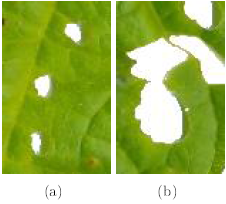
\includegraphics[width = 5cm]{./imgs/folhas.png}
	  \end{center}
	  \caption{Recortes em folíolos de soja: (a) Dano atribuído a um coleóptero; (b) Dano atribuído a uma lagarta.}
	\end{figure}

   \end{frame}

   \begin{frame}
    \frametitle{Introdução - Aplicação em Reconhecimento de Padrões}
	\begin{itemize}
		\item{Nosso problema requer um estudo sobre técnicas de reconhecimento de padrões necessarias à classificação de formas}
		\item{A literatura não possui trabalhos que tratam deste assunto específico (Classificação de danos em folíolos)}
		\item{Na revisão da literatura buscamos abordagens de classificação de formas em diversas aplicações}
		\item{O objetivo é adequar algumas delas ao nosso problema}
	\end{itemize}
   \end{frame}

  \section{Abordagens Atuais}
   \subsection{Similaridade de formas}
    
    \begin{frame}
     \frametitle{Similaridade de formas}
      \begin{itemize}
       \item{Passos:
	   \begin{enumerate}
		\item{Extração da borda do objeto}
		\item{Extrair características que estabeleçam critérios de similaridade entre as classes
		  \begin{itemize}
		   \item{Por Exemplo:Distancia entre o centro de massa e os pontos da borda} 
		  \end{itemize}
		}
		\item{Extração de partes menores da borda pela evolução da curva discreta ressaltando a similaridade de uma das classes}
	  \end{enumerate}	}
      \end{itemize}
    \end{frame}

    \begin{frame}
     \frametitle{Similaridade de formas}
      \begin{itemize}
       \item{Passos (Continuação):
	\begin{enumerate}
	  \setcounter{enumi}{3}
		\item{Constroi-se um conjunto de imagens com essas partes menores que serão comparadas no processo de classificação
		  \begin{itemize}
		    \item{Garante invariância à translação, rotação e escala} 
		  \end{itemize}
		}
	\end{enumerate}
       }
       \item{A disposição de nervuras nos folíolos atribui maior precisão a similaridade, aumentando a robustez do reconhecimento}
      \end{itemize}
    \end{frame}


   \subsection{Redes complexas}
     \begin{frame}
      \frametitle{Redes Complexas}
	\begin{itemize}
	 \item{Podem combinar algoritmos evolutivos que se aprimoram no treinamento de um perceptron geralmente aplicados em uma rede neuronal}
	 \item{Podem também representar o contorno da forma como uma rede complexa para posterior análise de sua complexidade}
	 \item{Metodologia utilizada no reconhecimento de folíolos de especies distintas, sendo invariante à escala, rotação e translação}
	\end{itemize}
     \end{frame}
     \begin{frame}
      \frametitle{Redes Complexas}

	\begin{figure}[h!]
	\centering
	  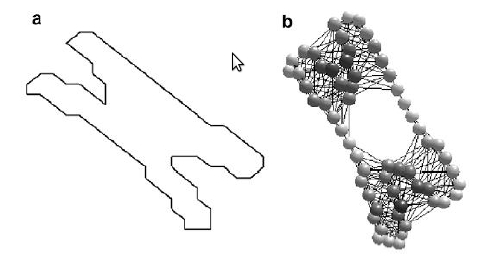
\includegraphics[width = 5 cm]{./imgs/rede.jpg}
	\caption{contorno modelado por uma rede complexa}
	\end{figure}


     \end{frame}


   \subsection{Algoritmos Genéticos}
     \begin{frame}
      \frametitle{Algoritmos Genéticos}
	\begin{itemize}
	 \item{Algoritmos genéticos são aplicados na etapa de \textit{matching}}
	 \item{Com isso o algoritmo associa mais precisamente as similaridades entre as imagens}
	 \item{A abordagem foi avaliada com extensos conjuntos de imagens, se mostrando invariante à translação, rotação e escala} 
	\end{itemize}
     \end{frame}
     \begin{frame}
      \frametitle{Algoritmos Genéticos}
      \begin{itemize}
       \item{Podem ser usadas várias maneiras de representação das características:
	  \begin{enumerate}
	    \Roman{enumi}
	    \item{Representar o contorno da folha como um grafo onde o peso é a angulação das curvas, e fazer o \textit{matching} pela comparação dos grafos}
	    \item{Geração de \textit{templates} para definir as classes que serão comparadas durante o \textit{matching}}
	  \end{enumerate}
	 }
      \end{itemize}
     \end{frame}

    
   \subsection{Outras Abordagens}
     \begin{frame}
      \frametitle{Outras Abordagens}
	\begin{enumerate}
	 \item{\textbf{\textit{Kernel-Edit Distance}} - É determinada pelo numero de operações para transformar um objeto em 
	    outro} 
	 \item{\textbf{Representação Simbólica} - O contorno da forma é representado através de um simbologia que garante 
	    invariância e robustez à extração de características}
	 \item{\textbf{Classificação pelo Esqueleto} - O \textit{matching} é feito sobre o esqueleto da forma}
	\end{enumerate}
     \end{frame}
     \begin{frame}
      \frametitle{Outras Abordagens}
	\begin{enumerate}
	 \setcounter{enumi}{3}
	 \item{\textbf{Forma Adaptativa e Segmentação Variacional} - Utilizada para reconhecimento de manuscritos históricos, 
	    se baseia em modelos pré-estabelecidos que se adaptam durante o segmentação e o \textit{matching}}
	 \item{\textbf{Equação de \textit{Poisson}} - Aplica-se a Equação de \textit{Poisson} sobre a silhueta do objeto
	    obtendo uma função que mostra o tempo gasto de cada ponto até a borda do objeto, sendo o método um eficiente descritor
	    de caracteristicas}
	\end{enumerate}

     \end{frame}


  \section{Conclusões}
    
   \begin{frame}
     \frametitle{Conclusões}
      \begin{itemize}
       \item{As abordagens apresentadas compõem o estado da Arte do problema de reconhecimento de formas}
       \item{As abordagens necessitam ser adaptadas ao nosso problema}
      \end{itemize}
   \end{frame}

   \begin{frame}
     \frametitle{Próximos Passos}
      \begin{itemize}
       \item{Implementar alguns dos métodos aqui apresentados}
       \item{Adequá-los ao nosso problema}
       \item{Efetuar testes sobre a nossa base de dados para estudar os resultados}
      \end{itemize}
   \end{frame}

   \begin{frame}
      \frametitle{Referências}
      \bibliographystyle{ieeetr}
      \bibliography{Bibliografia}
   \end{frame}

\end{document}